\documentclass{article}
\usepackage[utf8]{inputenc}
\usepackage[]{hyperref}

\author{
  Raatikka, Marko\\
  \texttt{marko.raatikka@aalto.fi}
  \and
  Lucas, Triefenbach\\
  \texttt{lucas.triefenbach@aalto.fi}
}
\title{Energy efficiency of HTTP2 over HTTP1.1 on the mobile web
\\
\vspace{5mm}
\large{CSE-E5440: Energy-efficient Mobile Computing\\Group C}
}
\date{\today}

\usepackage{natbib}
\usepackage{graphicx}

\begin{document}

\maketitle
\clearpage

\section{Part I}

\subsection{Introduction}
With the increasing computation power and connection speed of mobile phones in recent years, the amount of data flowing through the Internet to the consumer's end device continues to grow. While web applications have become ever more complex and the amount of HTML, JavaScript and CSS required to render a web page has grown, HTTP1.1 -- the prevailing transfer protocol of today's web -- has failed to keep up with the pace. One of the culprits of HTTP1.1 is that it can only handle one request per a TCP connection and that it can only have a certain maximum number of connections per host (5-8 connections depending on the browser). To work around these shortcomings developers have used techniques such as domain sharding (hosting assets across multiple domains), image spriting and inlining CSS \& JavaScript. However, a transport layer problem can not be efficiently solved at the application level.

The work for a new version of HTTP protocol was set forth by Google in 2012 in the form an open networking protocol called SPDY. Later, in 2015 , building on the work done for SPDY, HTTP2 was proposed as the future standard protocol. The biggest improvements HTTP2 introduces over HTTP1.1 are multiplexing of requests and responses to avoid a so called \emph{head-of-line blocking} inherent in HTTP1, header compression, prioritization of requests and server push mechanism. Web services are slowly migrating into adopting HTTP2, but as of today, only about 7\% of the websites have fully migrated to the new protocol. \citep{google-spdy}\citep{http2_stats}\citep{http2}

This work sets to study the impact of HTTP2 on mobile power consumption. Previous work on the topic has been done by \citep{previous_work}. However, this work focuses more on generating high traffic and mimicking common navigation patterns. Due to time constraints testing is limited to a single browser as opposed to testing across various versions. The content is organized as follows: chapter \ref{chapter:design-implementation} describes the method used, the testbed environment and the steps of a test run. Chapter \ref{chapter:results} continues by presenting the experiment results, which are later reviewed in Chapter \ref{chapter:discussion}. Last, an outline for the part II of the study is given.


\subsection{Design and Implementation}
\label{chapter:design-implementation}

The energy efficiency of the HTTP1.1 and HTTP2 protocols were measured by generating large amounts of network traffic. Six different web services were chosen as the targets, including Flickr, Yahoo, Facebook, Twitter, Weather.com and Instagram. These web services were selected based on their popularity and support for HTTP2 clients (browsers). Facebook, Twitter and Weather.com were eventually omitted from the final experiment corpus: the network traffic generated by Facebook was highly optimized, and therefore, it was assumed that it would not introduce any interesting differences in the payload sizes. Twitter on the other hand was deemed too lightweight (consisting of mostly text-based content), while Weather.com suffered from peculiar latency issues when transmitting images over HTTP2 as shown by Figure \ref{fig:weather.com}.

\begin{figure}[h!]
\centering
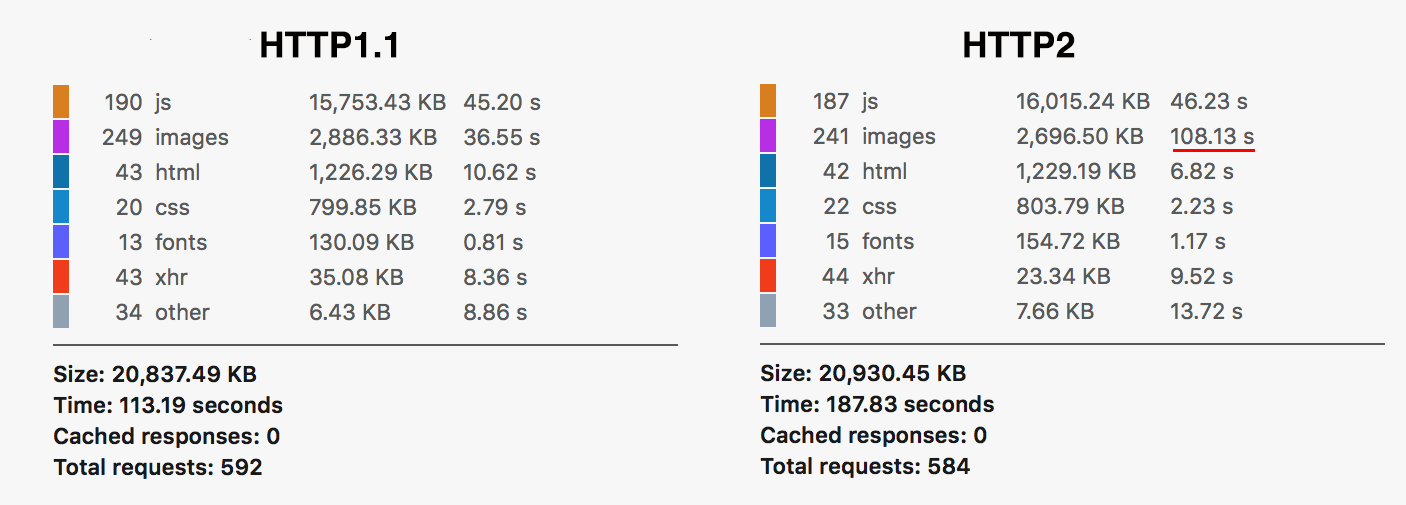
\includegraphics[scale=0.6]{images/weathercom.png}
\caption{Weather.com was excluded from the final experiment corpus because it exhibited abnormally long response times when image assets were fetched over HTTP2. This was done the prevent introducing bias to the energy consumption measurements.}
\label{fig:weather.com}
\end{figure}

The experiment was conducted using Firefox (version 42.0) as no other publicly available browsers support manually disabling HTTP2 support, as of this writing. The implementation of a robust and reproducible experiment environment required automation of the navigation logic. Browser automation frameworks Appium\footnote{Appium - \url{appium.io}} and Mozilla’s Robocop\footnote{Robocop - \url{https://wiki.mozilla.org/Auto-tools/Projects/Robocop}} were originally considered for this task. However, Appium lacked support for the Firefox browser, and Robocop -- Mozilla’s internal tool for testing Firefox on mobile -- missed proper documentation. Thus, an alternative approach -- including the use of Android’s low level input API -- was taken. The utilization of the input API was inspired by an open-source energy consumption measurement framework called GreenMiner \citep{greenminer}.

The Android input API allows for the emulation of device gestures, and consequently, automation of browser navigation. The trade-off of this approach is that it requires root access to the device. Therefore the Samsung S4 used for the experiment was rooted using ClockworkMod recovery (version 6.0.4.7) and CyanogenMod (version 12), which ships with Android 5.1.1. The upside of installing a custom ROM -- a customized OS image installed on the device's ROM memory -- like CyanogenMod is that any pre-installed Google services or bundled Samsung software were not installed in the phone. This helped in minimizing any unwanted power consumption generated by services running in the background unknowingly.

Monsoon Solutions' Power Monitor\footnote{\url{https://www.msoon.com/LabEquipment/PowerMonitor/}} was used for collecting the energy consumption data. The negative and positive terminals of the smartphone battery were connected to the power monitor using copper wire. The two reading terminals of the Samsung S4 battery were isolated with tape to allow the smartphone to be started using external power (the power monitor). The experiment scripts used for navigating to the different websites were implemented as Bash shell scripts. The scripts were transferred onto the device via USB using ADB (Android Debug Bridge). ADB also allowed controlling the execution of the test scripts from the laptop, so no human interaction was required while running the tests.

Prior to running the test suite different smartphone features that might have caused noise (e.g. power consumption of background processes) were disabled. This included disabling automatic brightness, notifications, sounds, vibrations, widgets, lights and any power saving features. Features enabled for experiment purposes were WiFi, Airplane mode and Developer options. The measurements were conducted in the Aalto open WiFi network during the late evening (22:00) to ensure low latency and minimal network congestion. All caching functionality of the Firefox browser was disabled to maximize network traffic (assets would always be fetched over the network). Crash reporting and monitoring capabilities of the browser were disabled so that they would not cause spikes in power consumption during the experiment. The browser HTTP2 support could be toggled on and off via the Firefox configuration interface. The cache and HTTP configuration flags used are listed in Table \ref{table:firefox_flags}. For further information the interested reader is referred to the MozillaZine Knowledge Base\footnote{MozillaZine Knowledge Base - \url{http://kb.mozillazine.org/}}.

\clearpage

\begin{table}[]
    \centering
    \begin{tabular}{l|c|}
        \textbf{Flag} & \textbf{Value} \\
        browser.cache.check\_doc\_frequency & 1 \\
        browser.cache.disk.enable           & FALSE \\
        browser.cache.memory.enable         & FALSE \\
        network.http.spdy.enabled.http2     & TRUE/FALSE
    \end{tabular}
    \caption{The Firefox configuration flags set in the experiment.}
    \label{table:firefox_flags}
\end{table}

After the smartphone and the laptop have been connected to the power monitor and the power measurement UI (Power Tool UI) has been opened the experiment is conducted as follows:

\begin{enumerate}
    \item Start the Power Monitor with an output voltage of 3.7V and sampling rate of 5000Hz
    \item Boot the phone and ensure it has been configured as described above
    \item Connect the smartphone to a laptop via its micro USB connection (for ADB communication)
    \item Install Firefox 46.0 via ADB and configure it as described above (partially automated)
    \item Execute the test suite \emph{n} number of times for either HTTP2 or HTTP1.1 (fully automated).
\end{enumerate}

Upon executing the test suite the power monitoring is manually started via the Power Tool UI for recording the energy consumption of the test run. The rundown of the \emph{test suite} is as follows:

\begin{enumerate}
    \item Close stale instances of Firefox (if any)
    \item Ensure brightness is set to maximum and no screen dim is enabled (a fail-safe mechanism)
    \item Upload experiment scripts to the phone via ADB
    \item Wait $t_{bwt}$ seconds and start Firefox (open at \emph{about:blank})
    \item Wait $t_{nwt}$ seconds and navigate to a target website
    \item Swipe down the page 3-4 times to force dynamic/lazily loaded content to be loaded waiting $t_{swt}$ seconds after each swipe
    \item Navigate to a subpage and wait $t_{nswt}$ seconds
    \item Repeat steps \textbf{6-7} for five different subpages
    \item Navigate to \emph{about:blank} and repeat steps \textbf{5-8} for each target website
    \item Wait $t_{nwt}$ seconds, close Firefox and wait $t_{bwt}$ seconds before concluding the experiment.
\end{enumerate}

The wait times referred to above are given in Table \ref{table:wait_times}. The tap wait time $t_{twt}$ was used when tapping was required for loading more page content (tapping on a \emph{Load more} button). In addition to running the test suite to gather energy consumption metrics, the test suite was also run separately to capture network traffic (payload sizes, latency, number of requests) via the Firefox WebIDE\footnote{Firefox WebIDE - \url{https://developer.mozilla.org/en-US/docs/Tools/WebIDE}}.

\begin{table}[h!]
    \centering
    \begin{tabular}{l|c|l|}
        \textbf{Variable} & \textbf{Duration (s)} & \textbf{Description} \\
        $t_{nwt}$   & 15    & Navigation wait time \\
        $t_{nswt}$  & 10    & Subpage navigation wait time \\
        $t_{bwt}$   & 5     & Base wait time \\
        $t_{swt}$   & 3     & Swipe wait time \\
        $t_{twt}$   & 2     & Tap wait time
    \end{tabular}
    \caption{Wait time variables used in the experiment.}
    \label{table:wait_times}
\end{table}

\subsection{Results}
\label{chapter:results}

The average network latency -- or Round Trip Time (RTT) -- and packet loss measured when connecting to the three target web services (Yahoo, Instagram, Flickr) via the Aalto open WiFi is presented in Table \ref{table:latency}.

\begin{table}[h!]
    \centering
    \begin{tabular}{c|c|c|c}
         \textbf{Web service} & \textbf{RTT (ms)} & \textbf{RTT std. dev (ms)} & \textbf{Packet loss} \\
        Yahoo   & 158 & 32 & 4.7\% \\
        Instagram  & 116 & 10 & 0.3\% \\
        Flickr & 132 & 12 & 0.3\% \\
    \end{tabular}
    \caption{RTT and packet loss experienced when being connected to the target websites via the Aalto open WiFi during the experiment.}
    \label{table:latency}
\end{table}

For both of the protocols (HTTP1.1 and HTTP2) the test suite was run three times. Figure \ref{fig:smoothed_power} visualizes the average power level for each of the test runs. The average is computed as a moving average using R\footnote{R: statistical computing framework - \url{https://www.r-project.org/}} and a generalized additive model (GAM) provided by the \emph{geom\_smooth()} function of the \emph{ggplot2}\footnote{ggplot2 - \url{http://docs.ggplot2.org/}} plotting library (version 2.1.0). As seen in the figure, it took 400 seconds for a single run of the test suite.

Figure \ref{fig:average_power} presents the power levels of a test run done over HTTP1.1. The samples (x-axis) have been averaged so that the average power level is calculated at intervals of 5000Hz (sampling rate of the Power Monitor). That is, each data point represents the average of a group of 5000 data points (power levels). The smoothed (moving) average is plotted for easier comparison. Observations made on the data are labeled with letters \emph{A-E}. These observations are discussed later in Chapter \ref{chapter:discussion}.

\begin{figure}[h!]
\centering
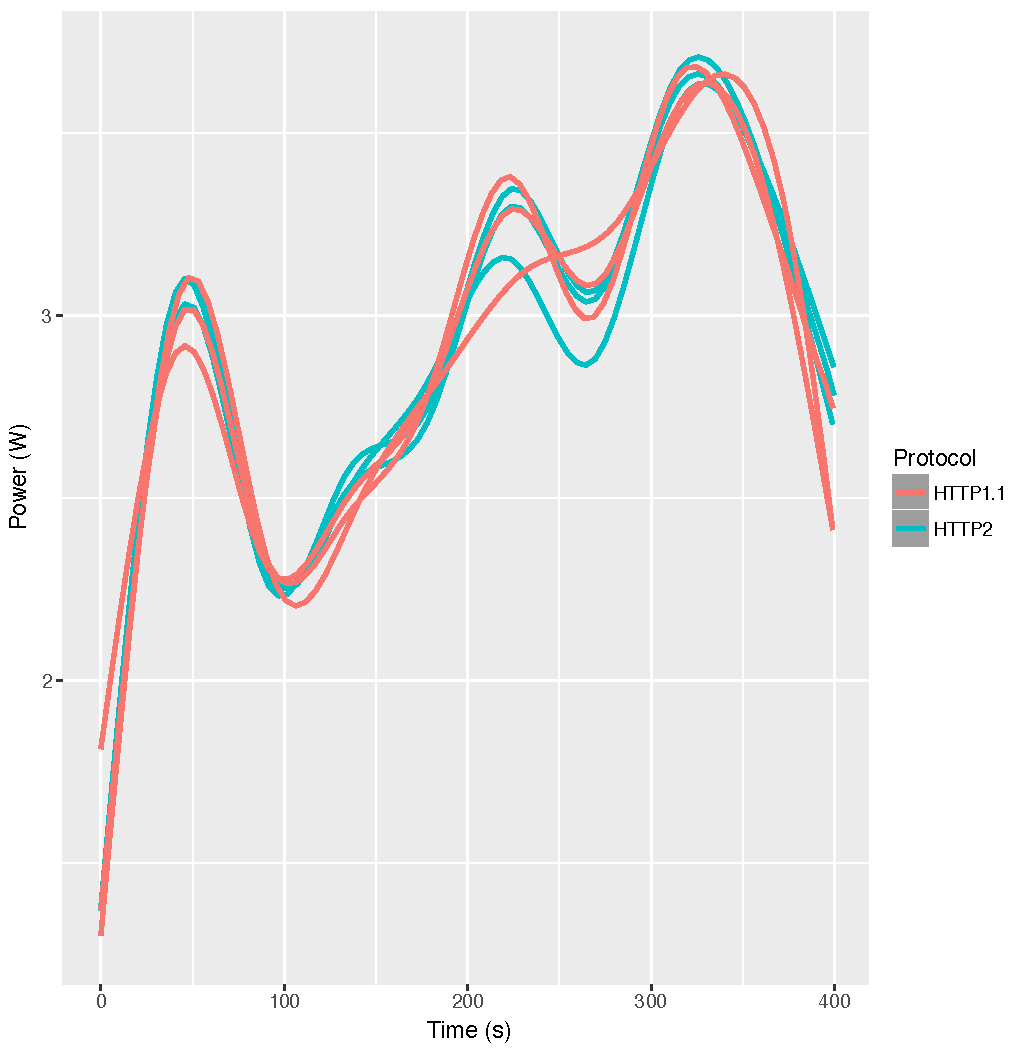
\includegraphics[scale=0.7]{images/smoothed_power}
\caption{Average power level of each test run with HTTP2 and HTTP1.}
\label{fig:smoothed_power}
\end{figure}

A summary of the mean power and total energy consumption of the three experiment runs for both HTTP2 and HTTP1.1 are given in Table \ref{table:energy_consumption}. The metrics are calculated for samples within the time frame of 24-395 seconds, which corresponds to the time when the first navigation is executed up until the time when navigating off to \emph{about:blank} after the last target website.

For more accurate analysis of the effect of network traffic, Figure \ref{fig:http2_network_traffic} provides a network request pie chart for the payload sizes, latency and number of requests for both HTTP2 and HTTP1.1. This data is based on a single run executed in addition to the actual experiment.

\begin{figure}[t]
\centering
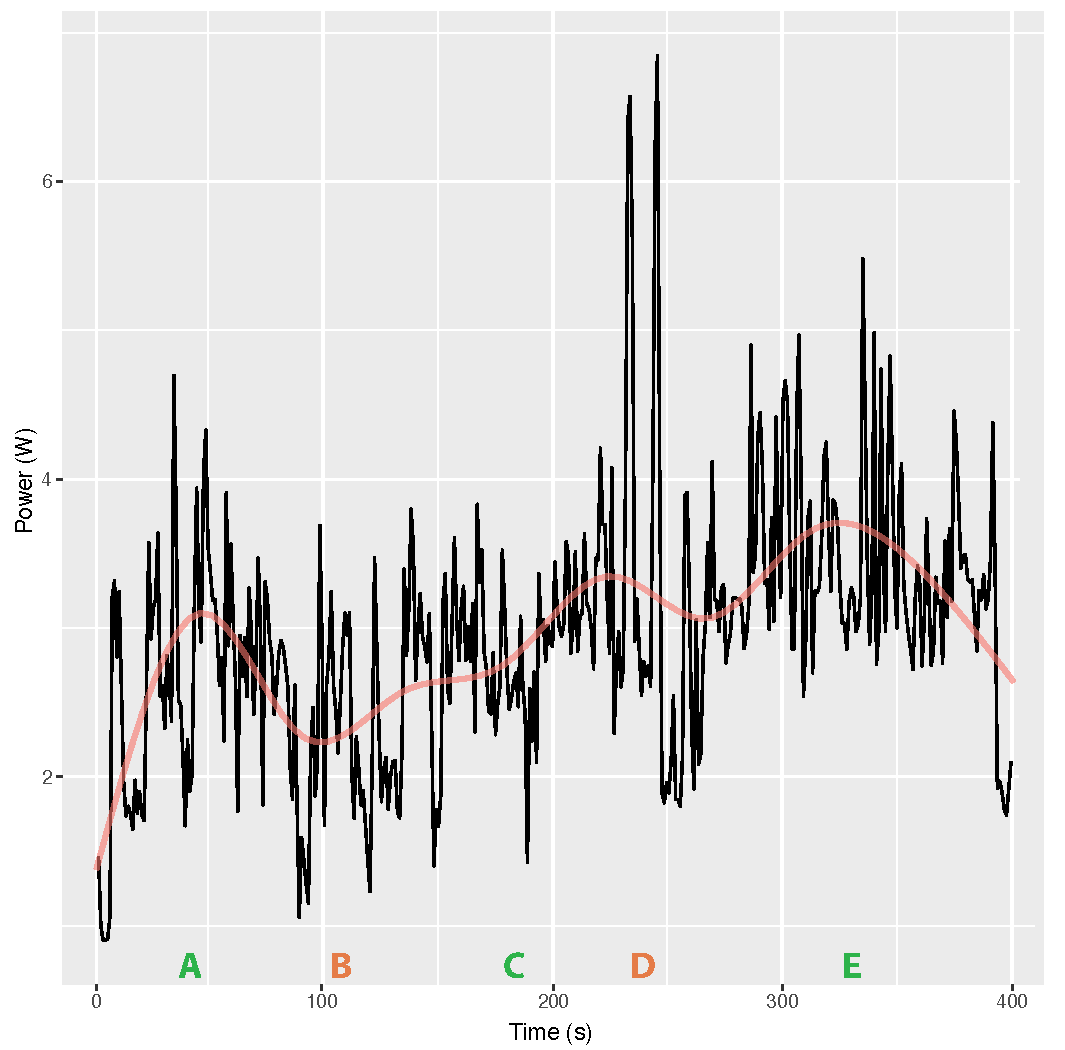
\includegraphics[scale=0.675]{images/average_power}
\caption{Average power levels (of every 1s segment) and the smoothed average of a test run done over HTTP1.1.}
\label{fig:average_power}
\end{figure}

\begin{table}[h!]
    \centering
    \begin{tabular}{c|c|c}
        & \textbf{HTTP1.1} & \textbf{HTTP2}  \\
        Mean (W)   & 2.987 & 2.995 \\
        Std.dev (W) & 0.984 & 1.007 \\
        Total (J)  & 1114.2 & 1117.2 \\
    \end{tabular}
    \caption{Energy consumption of HTTP1.1 and HTTP2 over the time frame of 24-395 seconds (from first navigation up until the exit navigation).}
    \label{table:energy_consumption}
\end{table}

\begin{figure}[h!]
\centering
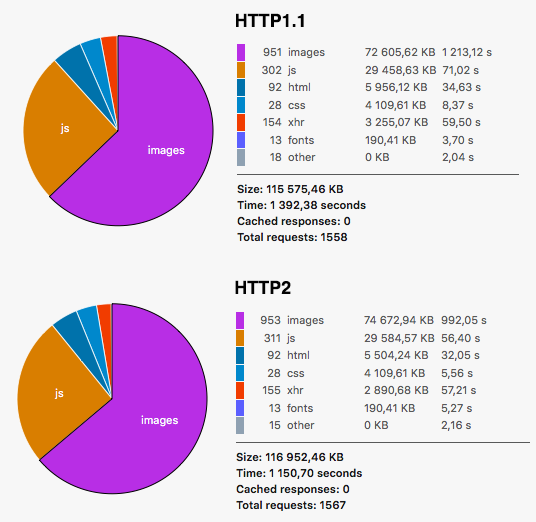
\includegraphics[scale=0.6]{images/http2_consumes.png}
\caption{The better latency of HTTP2 comes with the price of performance.}
\label{fig:http2_network_traffic}
\end{figure}

\clearpage

\subsection{Discussion}
\label{chapter:discussion}

DISCUSSION
    baseline power OS: 1 W \\
    app baseline power with Browser: 1.8 W \\
    talk about ENERGISE (\url{https://github.com/ds4se/chapters/blob/master/abramhindle/energymining.md#Hindle2014})
    interpretation of results (explain A-E)
    outline for part II

navigation order not randomized

network environment (why WiFi and not 2G, 3G, latency table in Google Drive)
Wifi is the only type of networking used in the setup for the following reason.
Different types of connections were tested and in the testing location 2G resulted in a high paket loss, which made 2G incomparable to the other types. While 3G and 4G did not display any difference in latency and package loss, than the wifi connected to the aalto-open network. This may be due to the setup station being located near the mobile providers antennas, which are on the roof of the CS building. For this reason only wifi was used in the testing setup. Another factor that might have an influence on the latency is that all readings were taken in the evening, when the building was nearly empty. This results in low latency, since all networks have low loads in general. On the other hand testig during the day might lead to biased results because of higher load fluctuations in the networks.

\section{Part II}

\emph{Evaluation of potential power saving mechanisms...}

\subsection{Proposal for Improvements}
TBD

\subsection{Conclusions}
TBD

\bibliographystyle{plain}
\bibliography{references}
\end{document}
